\chapter{Requirement definitions}

Building on the foundational definitions and technical frameworks previously discussed, this chapter offers an in-depth overview of our project, the Ilef Unified Cloud Management Platform. We start by examining the requirements to outline the essential functional and non-functional specifications critical for the platform’s design and implementation. Next, we will construct the Product Backlog to steer our project goals. Lastly, we will illustrate the primary use cases for the platform, highlighting its capability to enable efficient management and interoperability among various cloud providers and services.


\pagebreak

\section{Requirements analysis}

%\subsection{Design session}
%After  the beginning of the internship, we had a on-month training where we were
%trained about the different technologies that Pulpetech is using, such as Django, Angular, PostgreSQL.. %technologies
%Also, as interns, we had the opportunity, first, to get
%familiar with the company's working environment, second, understand better the
%project's goal and its added value to its users, and third, were able to collect
%the functional and non functional requirements of the project.
\subsection{Functional Requirements}
The overall goal of this project is to develop a comprehensive dashboard for real-time management and monitoring of cloud resources, specifically tailored to support the operational needs of Ilef. The platform is designed exclusively for use by Cloud/DevOps engineers, providing detailed control and oversight of various cloud environments. The following functionalities are essential:

\subsubsection{Initial Setup and Configuration}
Before utilizing the main features of the dashboard, the following servers must be deployed and configured:
\begin{itemize}
    \item \textbf{Jira}: For project management.
    \item \textbf{Mattermost}: For team communication.
    \item \textbf{Glitchtip}: For error and performance monitoring.
    \item \textbf{Jenkins}: For automating builds and deployment pipelines.
    \item \textbf{Vault}: For managing and securing secrets.
    \item \textbf{Nexus}: For storing and managing Docker images and other artifacts.
    \item \textbf{SonarQube}: For continuous inspection of code quality.
\end{itemize}

\subsubsection{Core Functionalities}
The dashboard provides several critical functionalities for the Cloud/DevOps engineer:
\begin{itemize}
    \item \textbf{Authentication}: Ensure secure access to the platform, allowing only authorized Cloud/DevOps engineers to log in and interact with the system.
    \item \textbf{Virtual Machine Management}: Enable the manual provisioning, configuration, and management of virtual machines across multiple cloud providers, including AWS, Azure, GCP, and Hetzner. This includes starting, stopping, restarting, and deleting virtual machines.
    \item \textbf{Bucket Management}: Allow engineers to manually upload, retrieve, and delete objects within storage buckets across AWS, Azure, and GCP, providing flexible data management options.
    \item \textbf{Docker Image Management}: Facilitate the uploading of Docker images directly to virtual machines and support the creation of Kubernetes clusters from these images for container orchestration.
    \item \textbf{Nexus Repository Operations}: Enable easy retrieval of Docker images stored in the Nexus repository, facilitating efficient image management and deployment.
    \item \textbf{Vault Secret Management}: Provide secure access to and management of secrets stored in the Vault server, essential for the configuration and operation of applications and infrastructure.
    \item \textbf{Scrumboard Management}: Integrate a Scrumboard within the platform that allows Cloud/DevOps engineers to create, update, and track tasks throughout the development cycles, enhancing organizational capabilities and project tracking.
\end{itemize}

\subsubsection{Building Advanced Visualization Tools}
To support effective resource management, the platform includes advanced visualization tools:
\begin{itemize}
    \item \textbf{Interactive Data Visualization}: Develop a dashboard that provides interactive charts and graphs detailing current resource usage, historical data, and predictive analytics, enabling users to interact with the data and gain new insights.
    \item \textbf{Customizable Data Views}: Allow users to customize views and filters to display data based on various parameters such as resource type, usage statistics, and provider, enhancing their ability to monitor and manage resources effectively.
\end{itemize}

\subsection{Non-Functional Requirements}

\subsubsection{Performance}
\begin{itemize}
    \item \textbf{Efficiency}: The platform should manage operations like virtual machine administration, bucket handling, and Docker image processing swiftly and with minimal latency.
    \item \textbf{Response Time}: Tasks such as starting or stopping a virtual machine should complete within a few seconds.
    \item \textbf{Throughput}: The system needs to handle multiple simultaneous operations efficiently, ensuring high throughput and minimizing user wait times.
    \item \textbf{Scalability}: The platform must scale effectively to manage increased loads, allowing numerous users to perform tasks concurrently without significant performance loss.
\end{itemize}

\subsubsection{Reliability}
\begin{itemize}
    \item \textbf{System Stability}: The platform should deliver consistent performance and maintain high reliability with minimal downtime.
    \item \textbf{Maintenance}: Conduct maintenance during off-peak hours and notify users in advance to minimize disruptions.
    \item \textbf{Monitoring and Alerts}: Establish thorough monitoring and alerting mechanisms to quickly identify and resolve issues, ensuring continuous operation and minimal downtime.
    \item \textbf{Data Integrity}: Maintain data integrity by detecting and preventing unauthorized modifications.
\end{itemize}

\subsubsection{Maintainability}
\begin{itemize}
    \item \textbf{Modular Architecture}: Develop the system using a modular architecture to facilitate easy updates, maintenance, and scalability.
    \item \textbf{Logging and Monitoring}: Implement detailed logging and monitoring systems to promptly identify and address issues, ensuring the platform's overall health and performance.
\end{itemize}


\section{Requirement specifications}
\subsection{Actors Identification}

The Ilef management platform is designed for Cloud/DevOps engineers and administrators, each with distinct roles and responsibilities within the system.

\subsubsection{User Roles}

\paragraph{Cloud/DevOps Engineer}
\begin{itemize}
    \item \textbf{Role Description}: This user primarily engages with the platform to oversee and manage cloud resources and will be referred to as \textbf{"User"} throughout the rest of the report.
    \item \textbf{Key Functions}:
    \begin{itemize}
        \item Log in and authenticate
        \item Administer virtual machines on AWS, Azure, GCP, and Hetzner
        \item Manage objects in cloud storage buckets on AWS, Azure, and GCP (upload, fetch, delete)
        \item Deploy Docker images to virtual machines
        \item Set up Kubernetes clusters from Docker images
        \item Retrieve Docker images from the Nexus repository
        \item Access secrets stored in the Vault server
        \item Use the Scrumboard for task management
    \end{itemize}
\end{itemize}

\paragraph{Administrator}
\begin{itemize}
    \item \textbf{Role Description}: This user has comprehensive access to all platform features, including advanced user management functions.
    \item \textbf{Key Functions}:
    \begin{itemize}
        \item Perform all functions available to Cloud/DevOps Engineers
        \item Create, modify, and delete user accounts
    \end{itemize}
\end{itemize}


\subsection{Use cases diagrams}
\begin{itemize}

    \item The following figure  \hyperref[fig:general_use_cases]{\ref{fig:general_use_cases}} introduces the general use cases which present the
functionalities of the application.

\begin{figure}[htbp]
  \center
  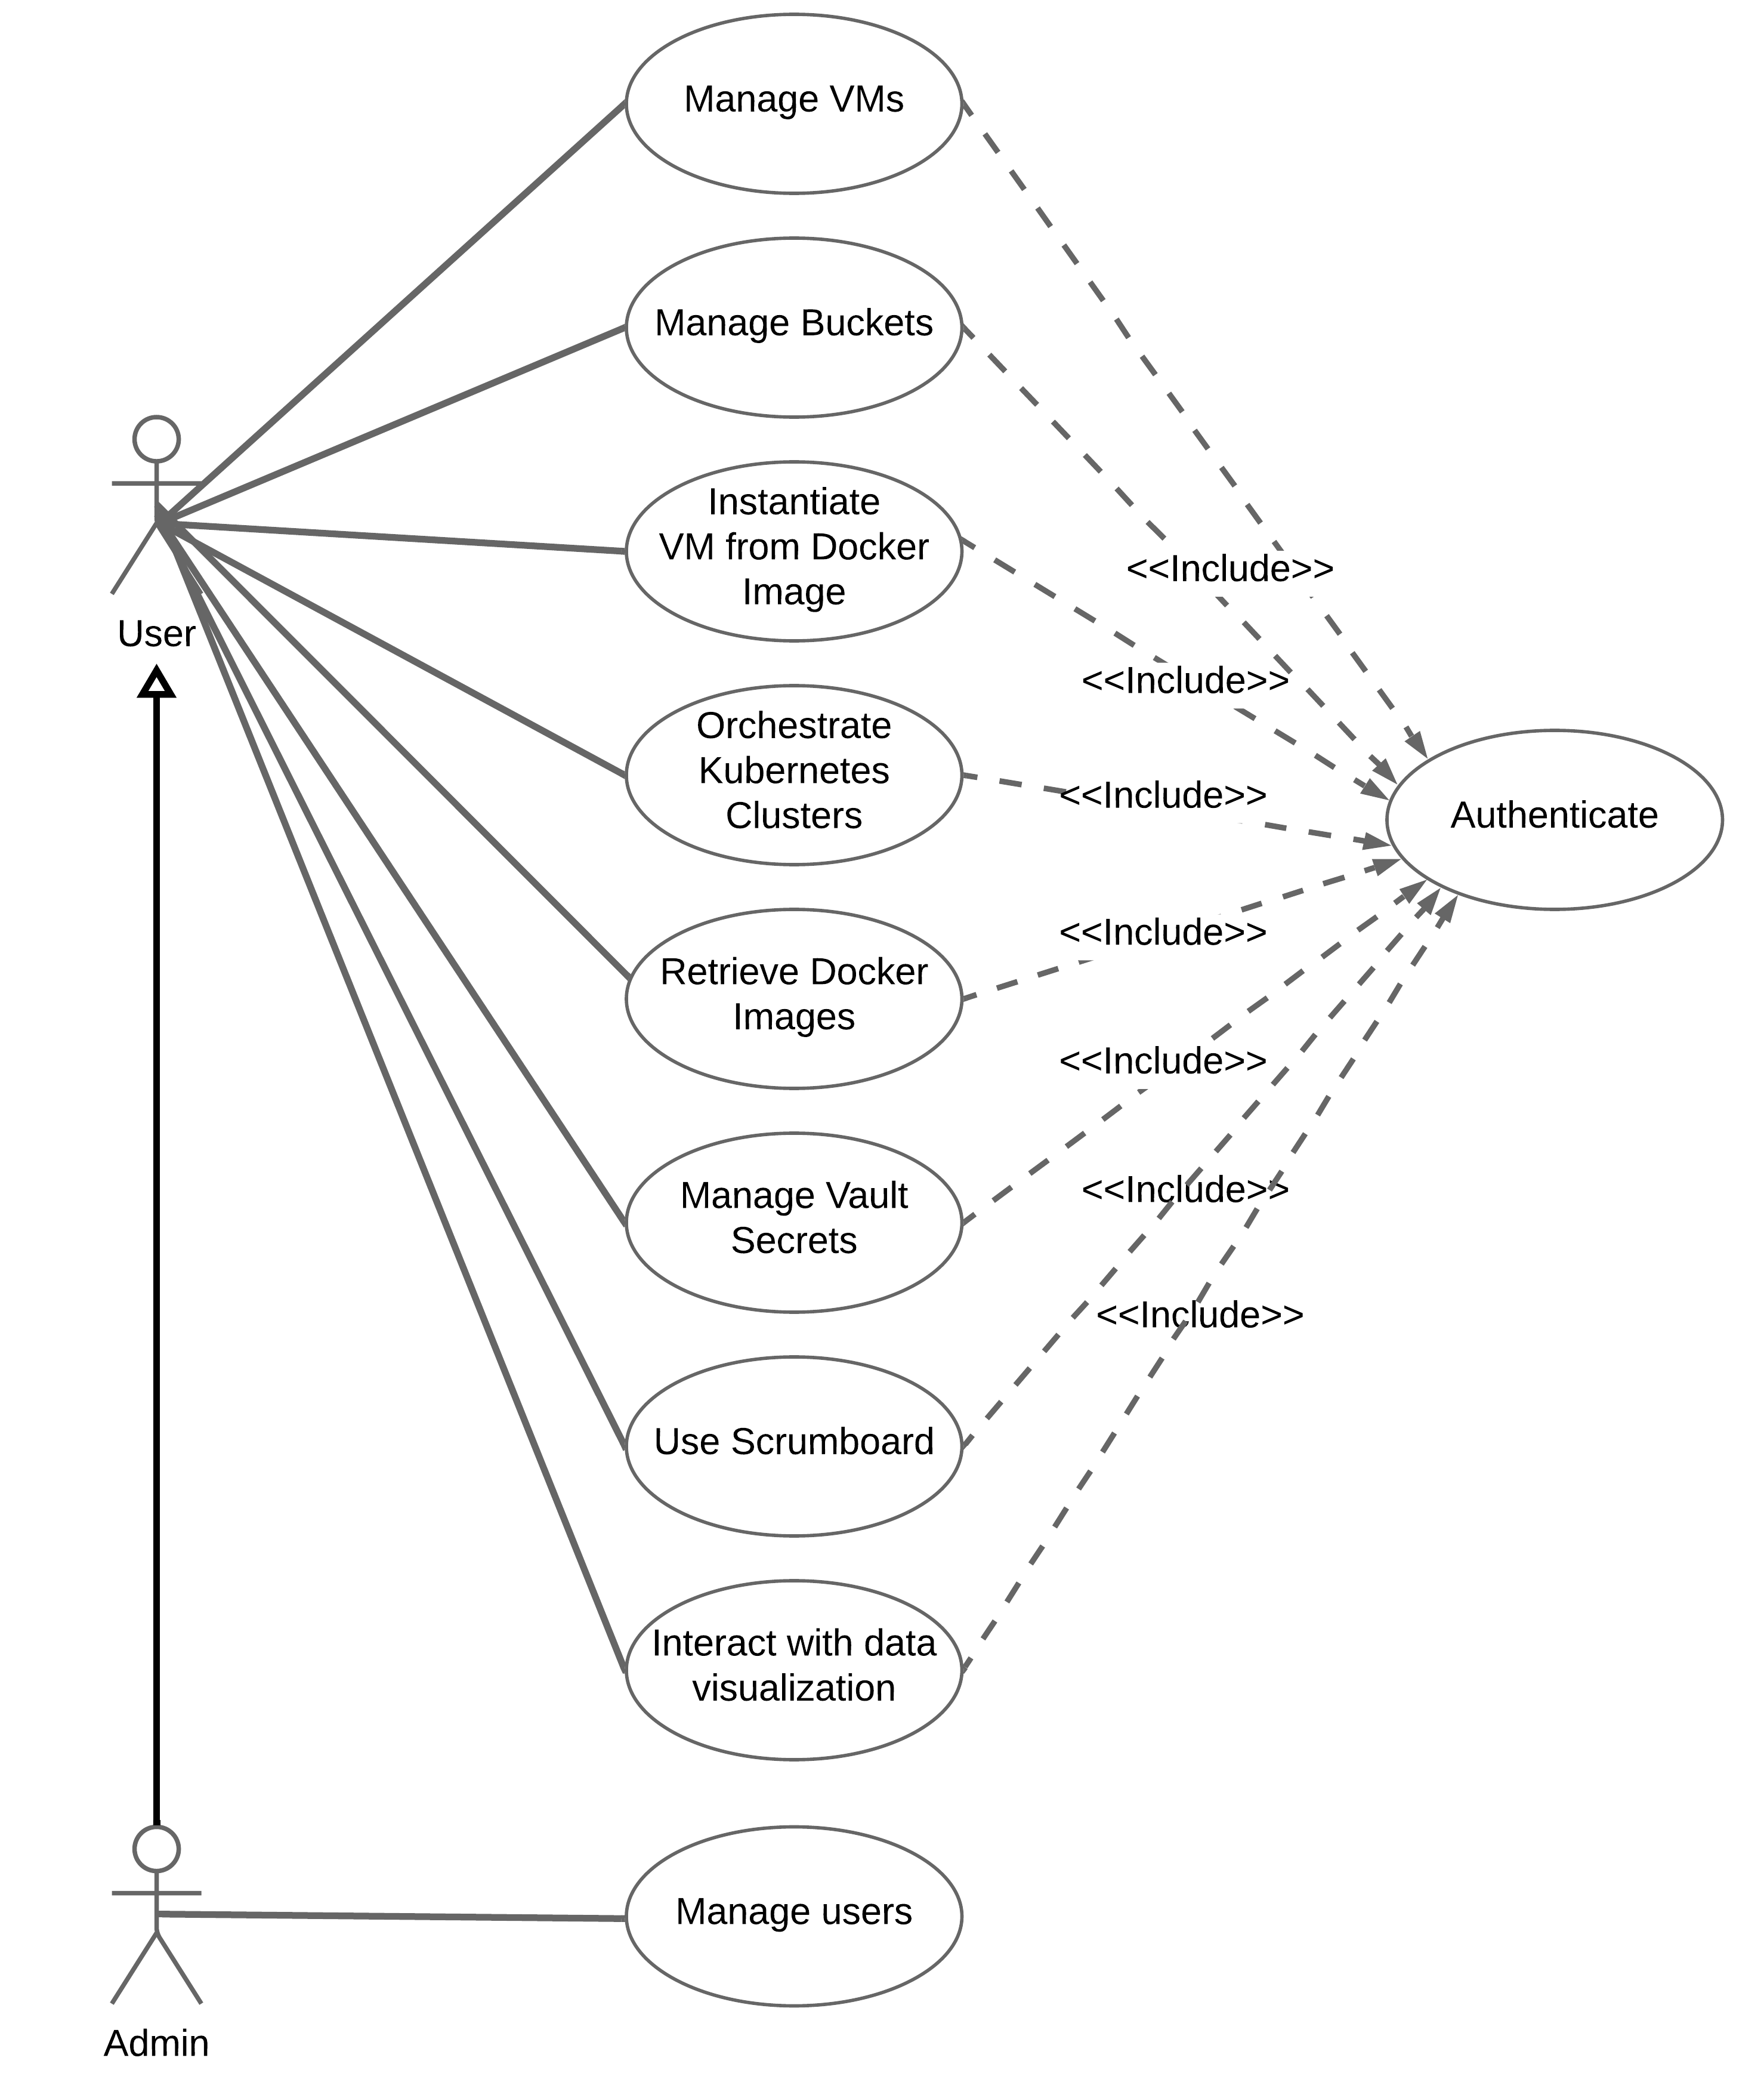
\includegraphics[width=19cm]{general_use_cases}
  \caption{General use case diagram}
  \label{fig:general_use_cases}
\end{figure}
\vspace{170mm}
\item The figure below (\hyperref[fig:use_case-manage_vm2]{Figure \ref{fig:use_case-manage_vm2}}) illustrates the ``Manage VMs'' detailed use case.
\vspace{-0.2in}
\begin{center}
\begin{figure}[h]
  \center
%\hspace*{-0.9in}
  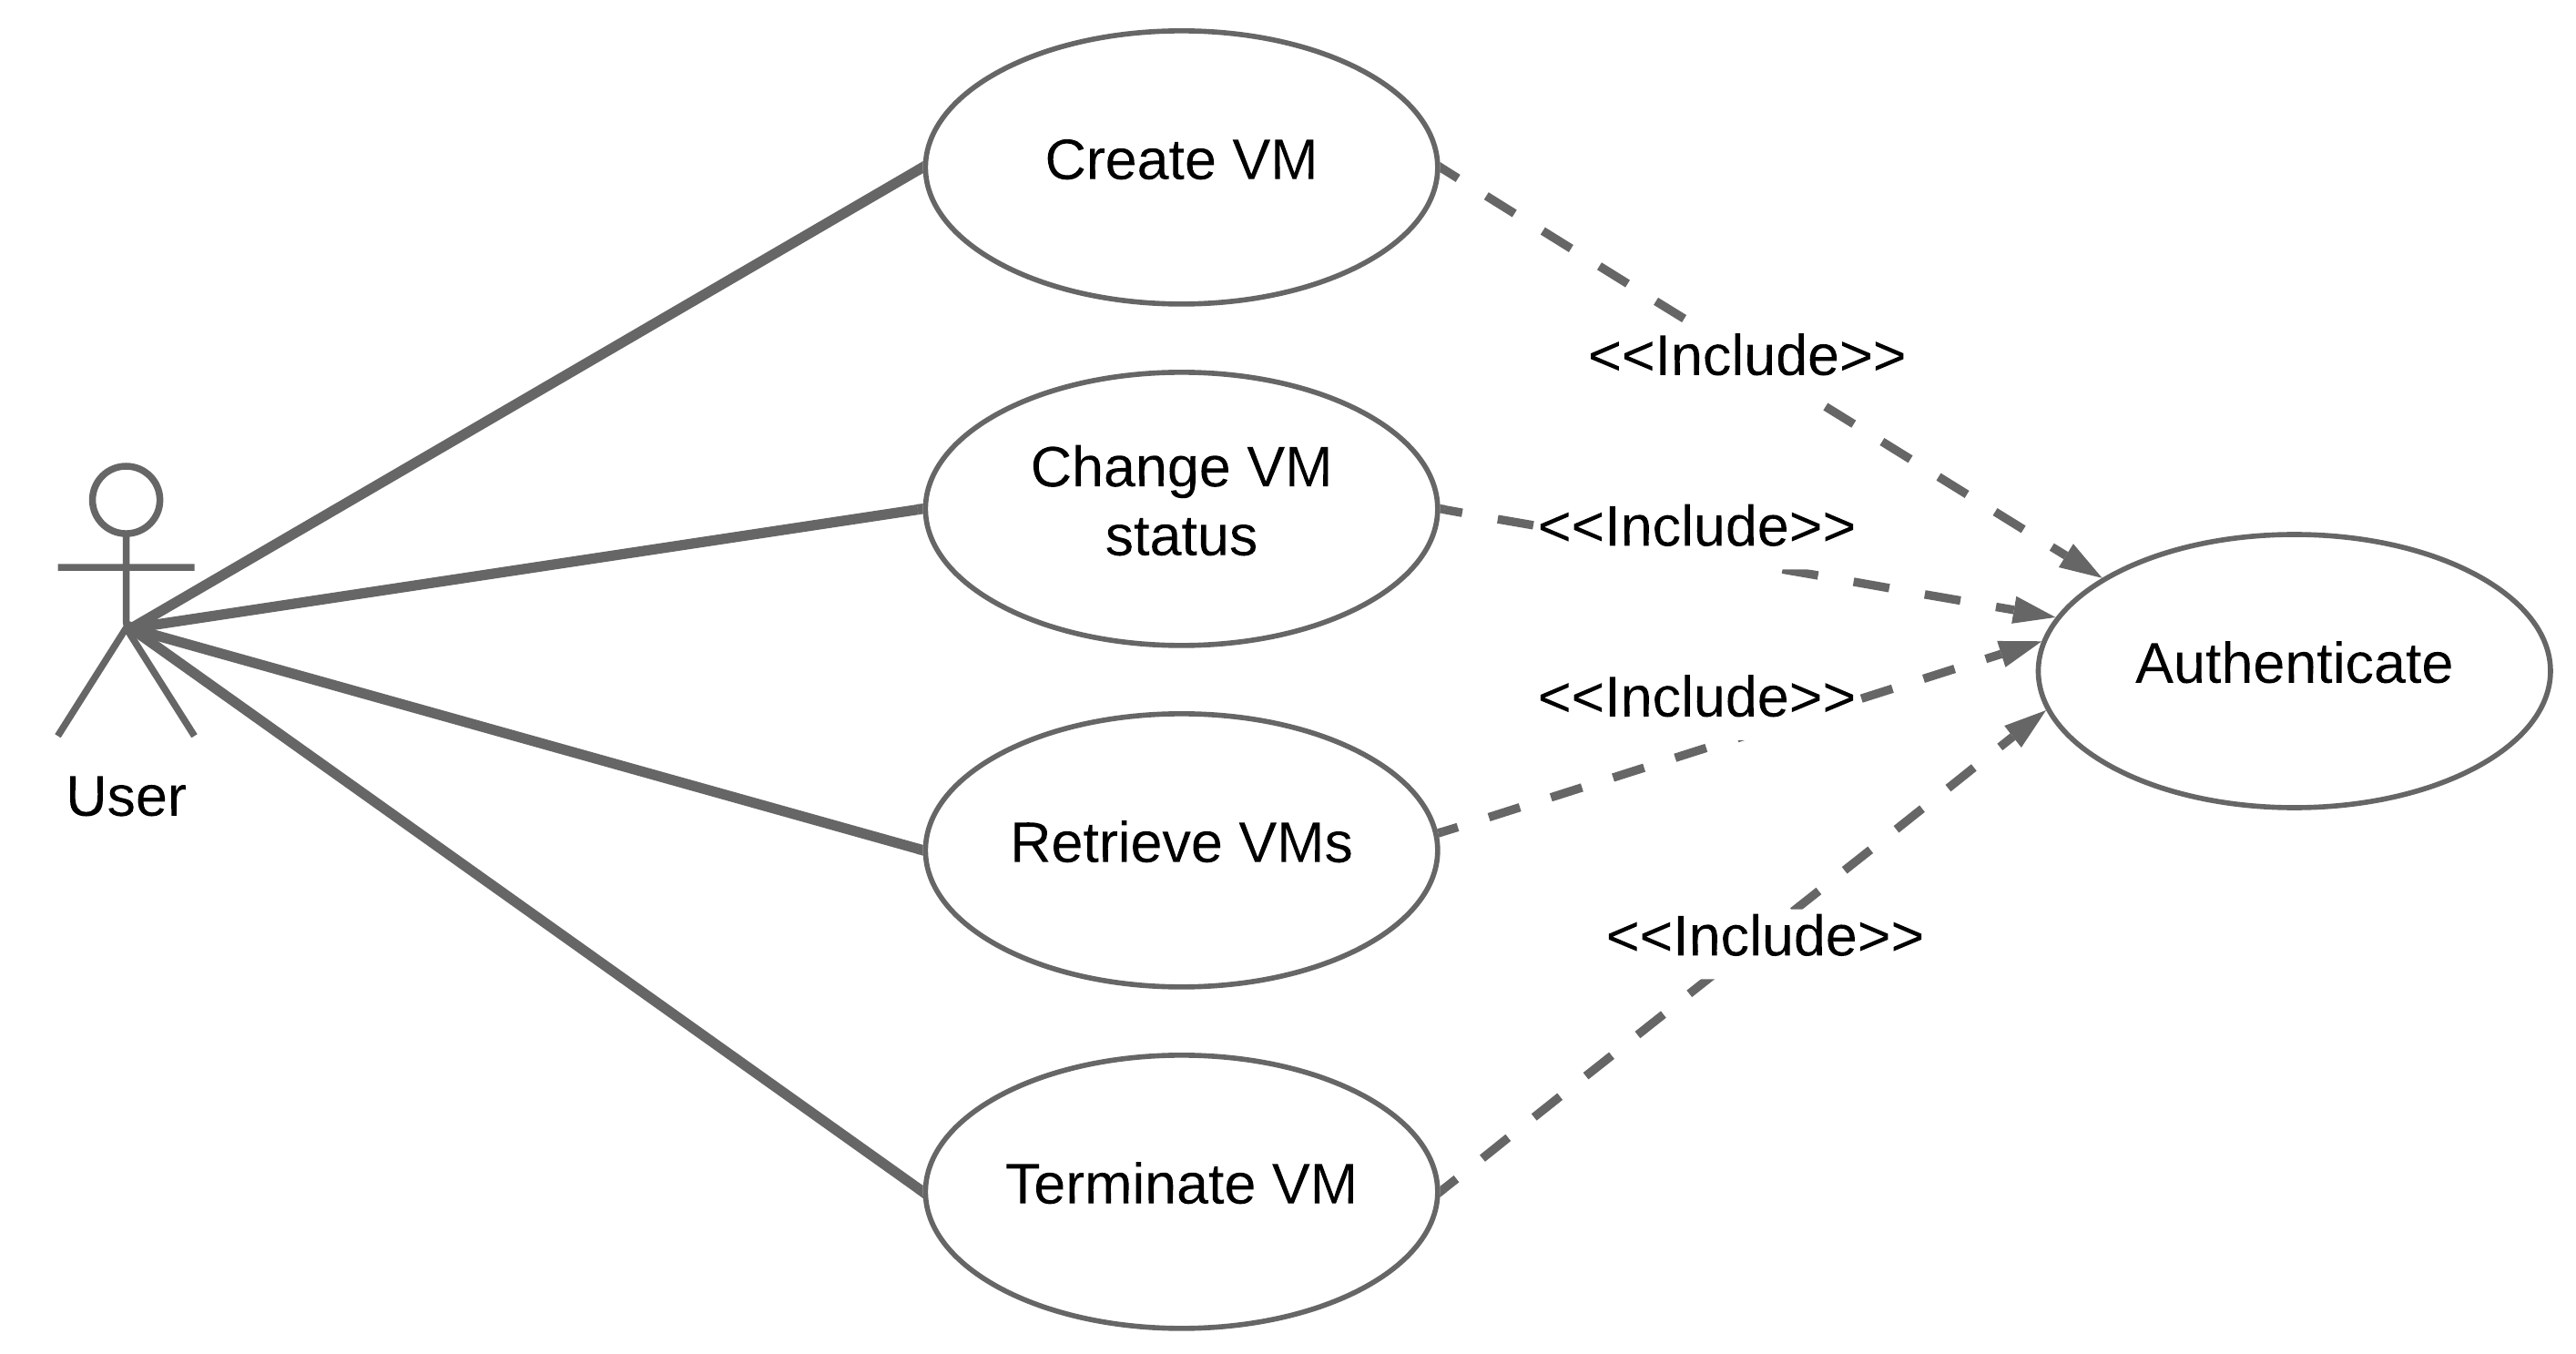
\includegraphics[width=15cm]{use_case-manage_vm2}
  \caption{Manage VMs detailed use case diagram}
  \label{fig:use_case-manage_vm2}
\end{figure}
\end{center}
\item The figure (\hyperref[fig:use_case-manage_vault]{Figure \ref{fig:use_case-manage_vault}})  shows the ``Manage Vault Secrets'' detailed use case.
\begin{center}
\begin{figure}[htbp]
  \center
% \hspace*{-0.9in}
  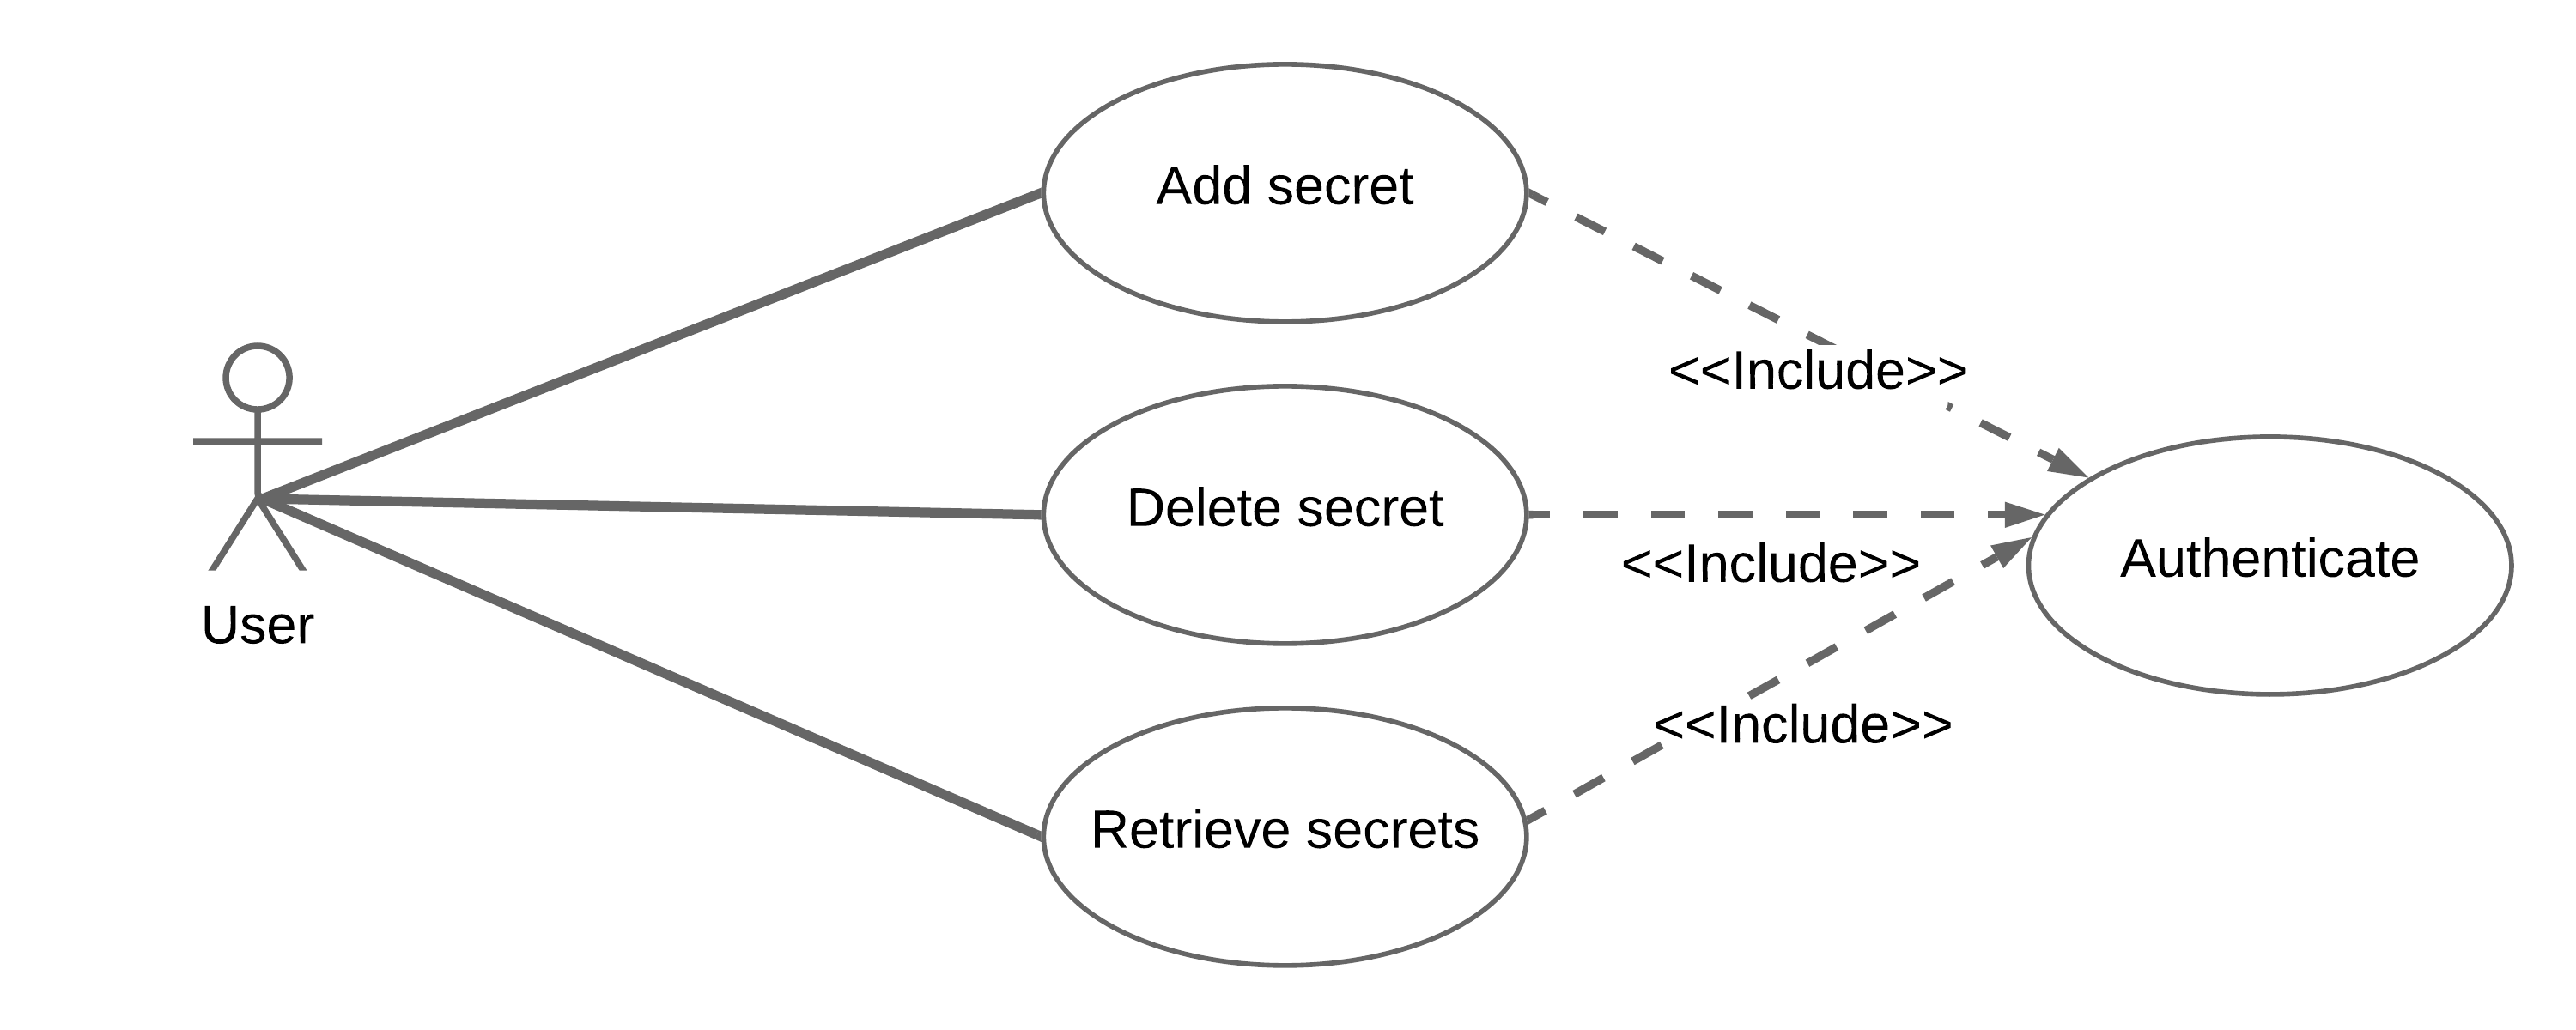
\includegraphics[width=15cm]{use_case-manage_vault}
  \caption{Manage Vault Secrets detailed use case diagram}
  \label{fig:use_case-manage_vault}
\end{figure}
\end{center}

\vspace{150mm}
\item The following figure (\hyperref[fig:use_case-manage_bucket2]{Figure \ref{fig:use_case-manage_bucket2}}) illustrates the detailed use case for ``Manage Buckets''.


\begin{figure}[h]
  \center
%\hspace*{-0.9in}
  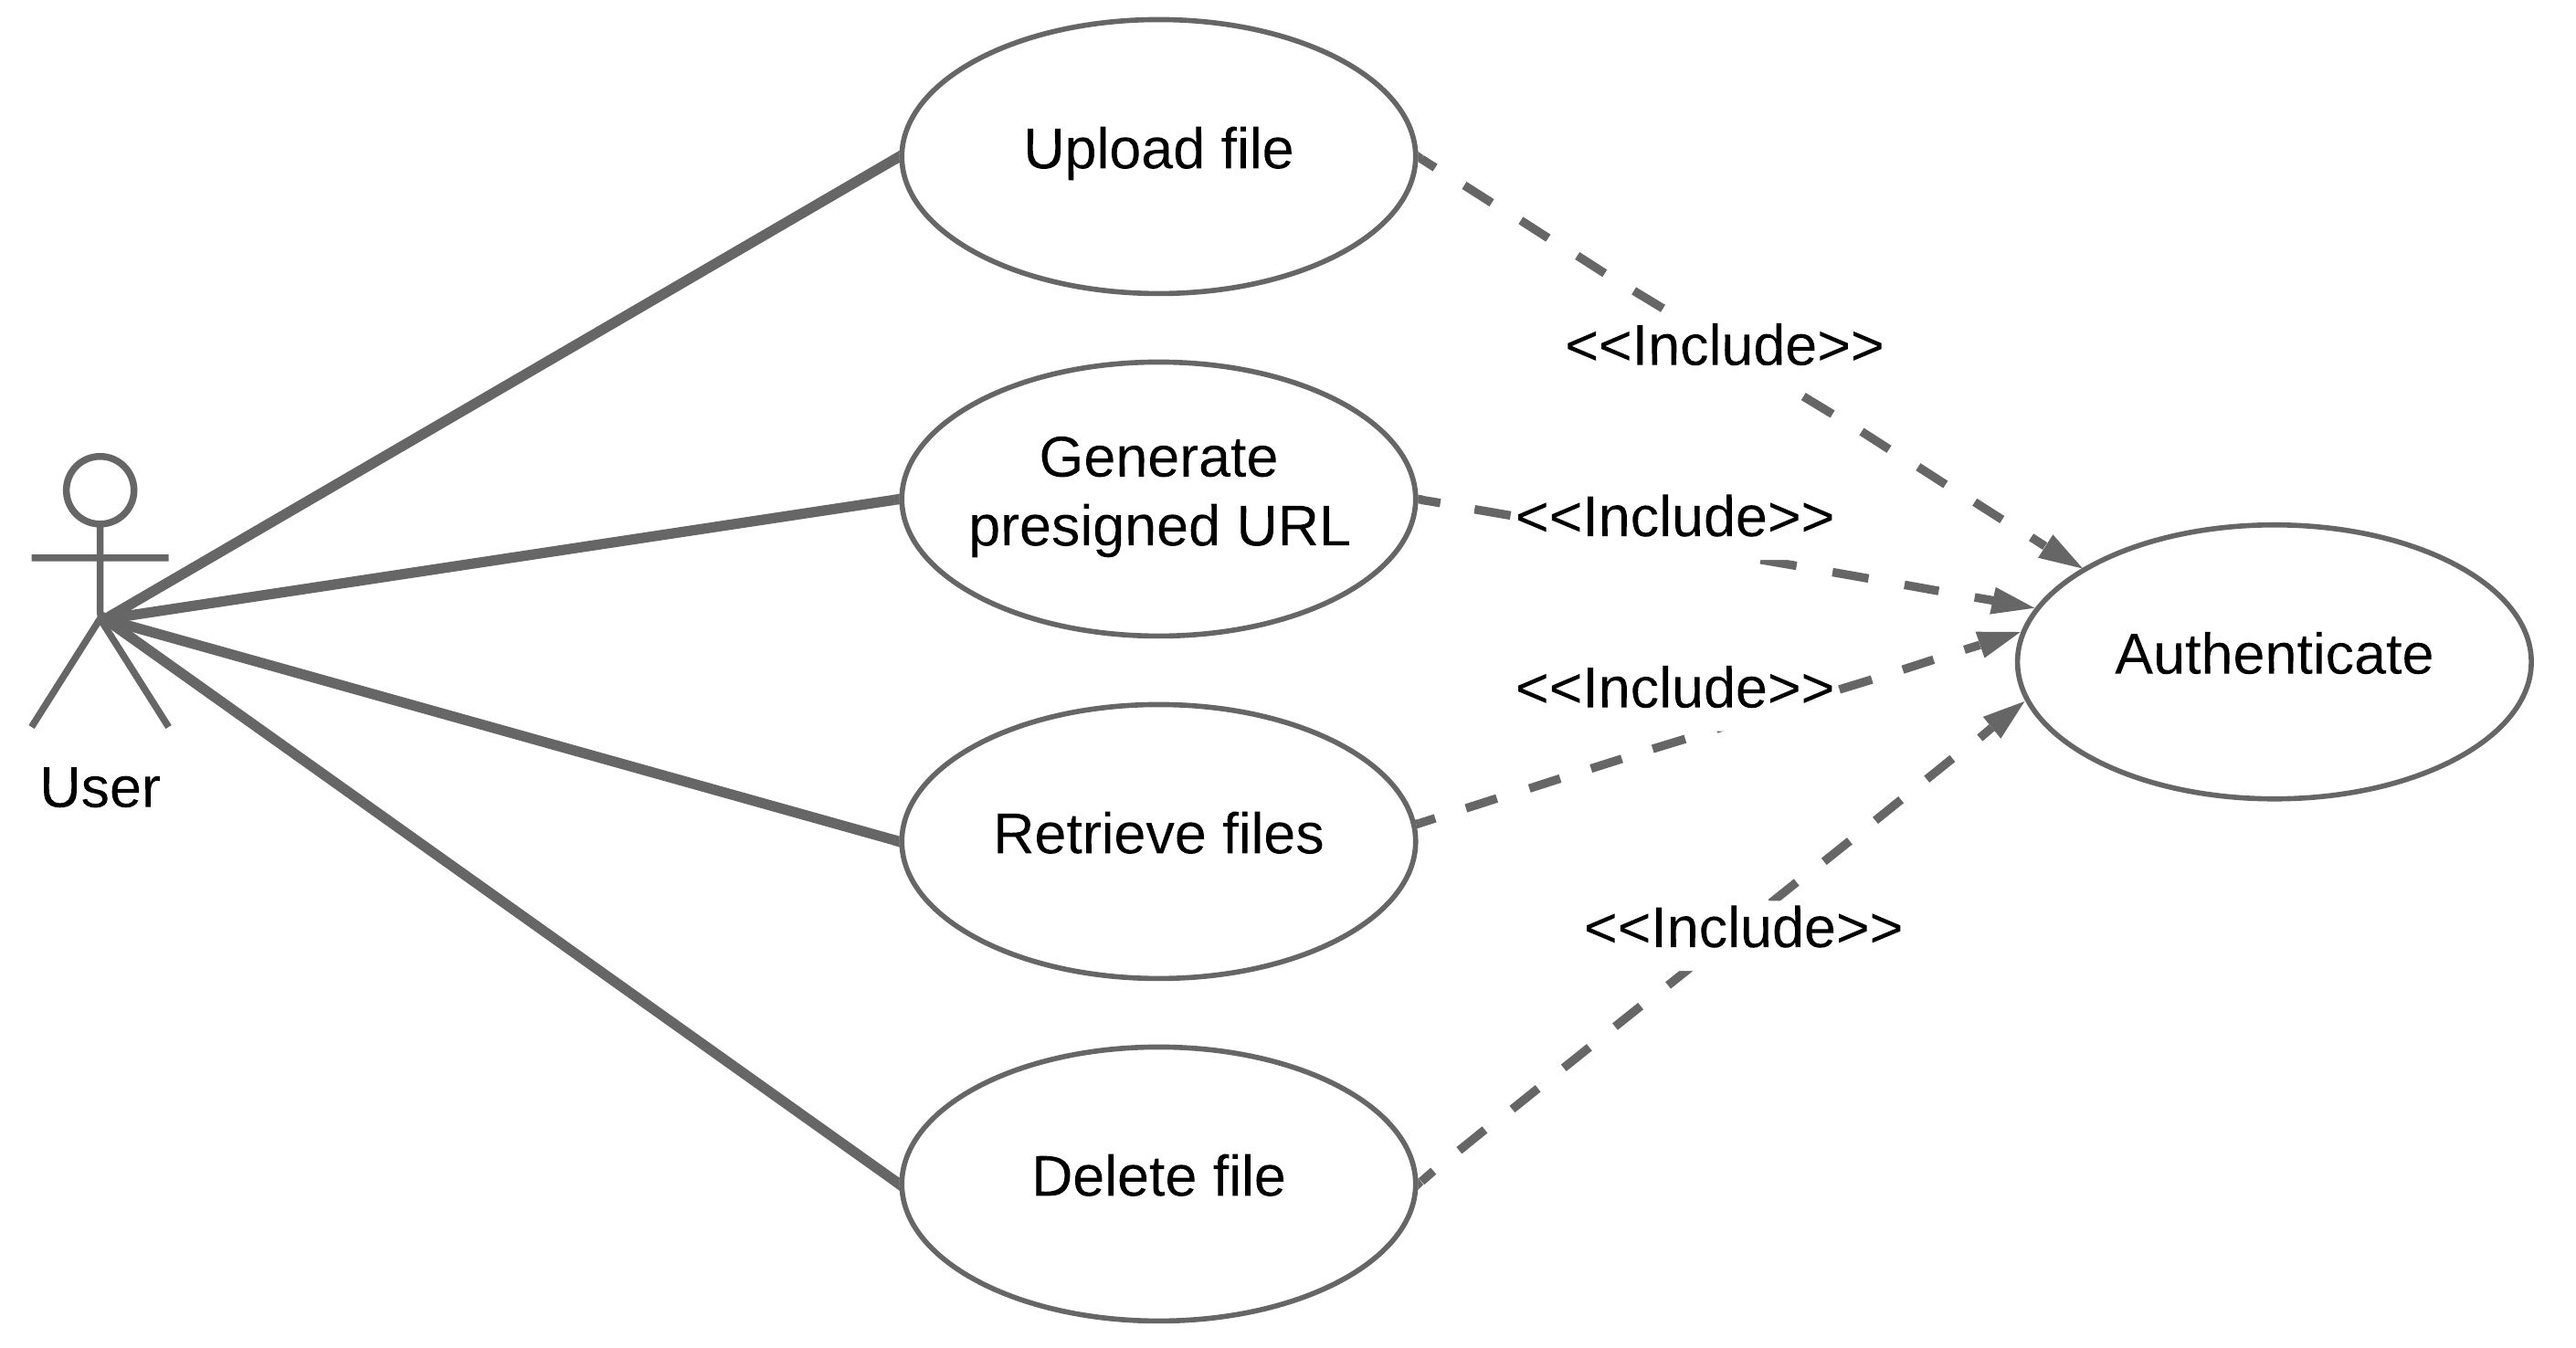
\includegraphics[width=15cm]{use_case-manage_bucket2}
  \caption{Manage Buckets detailed use case diagram}
  \label{fig:use_case-manage_bucket2}
\end{figure}

% \end{itemize}

\item The following figure (\hyperref[fig:use_case-manage_users2]{Figure \ref{fig:use_case-manage_users2}})  represents the admin ``Manage users'' detailed use case.
\vspace{150mm}
\begin{figure}[h]
  \center
%\hspace*{-0.9in}
  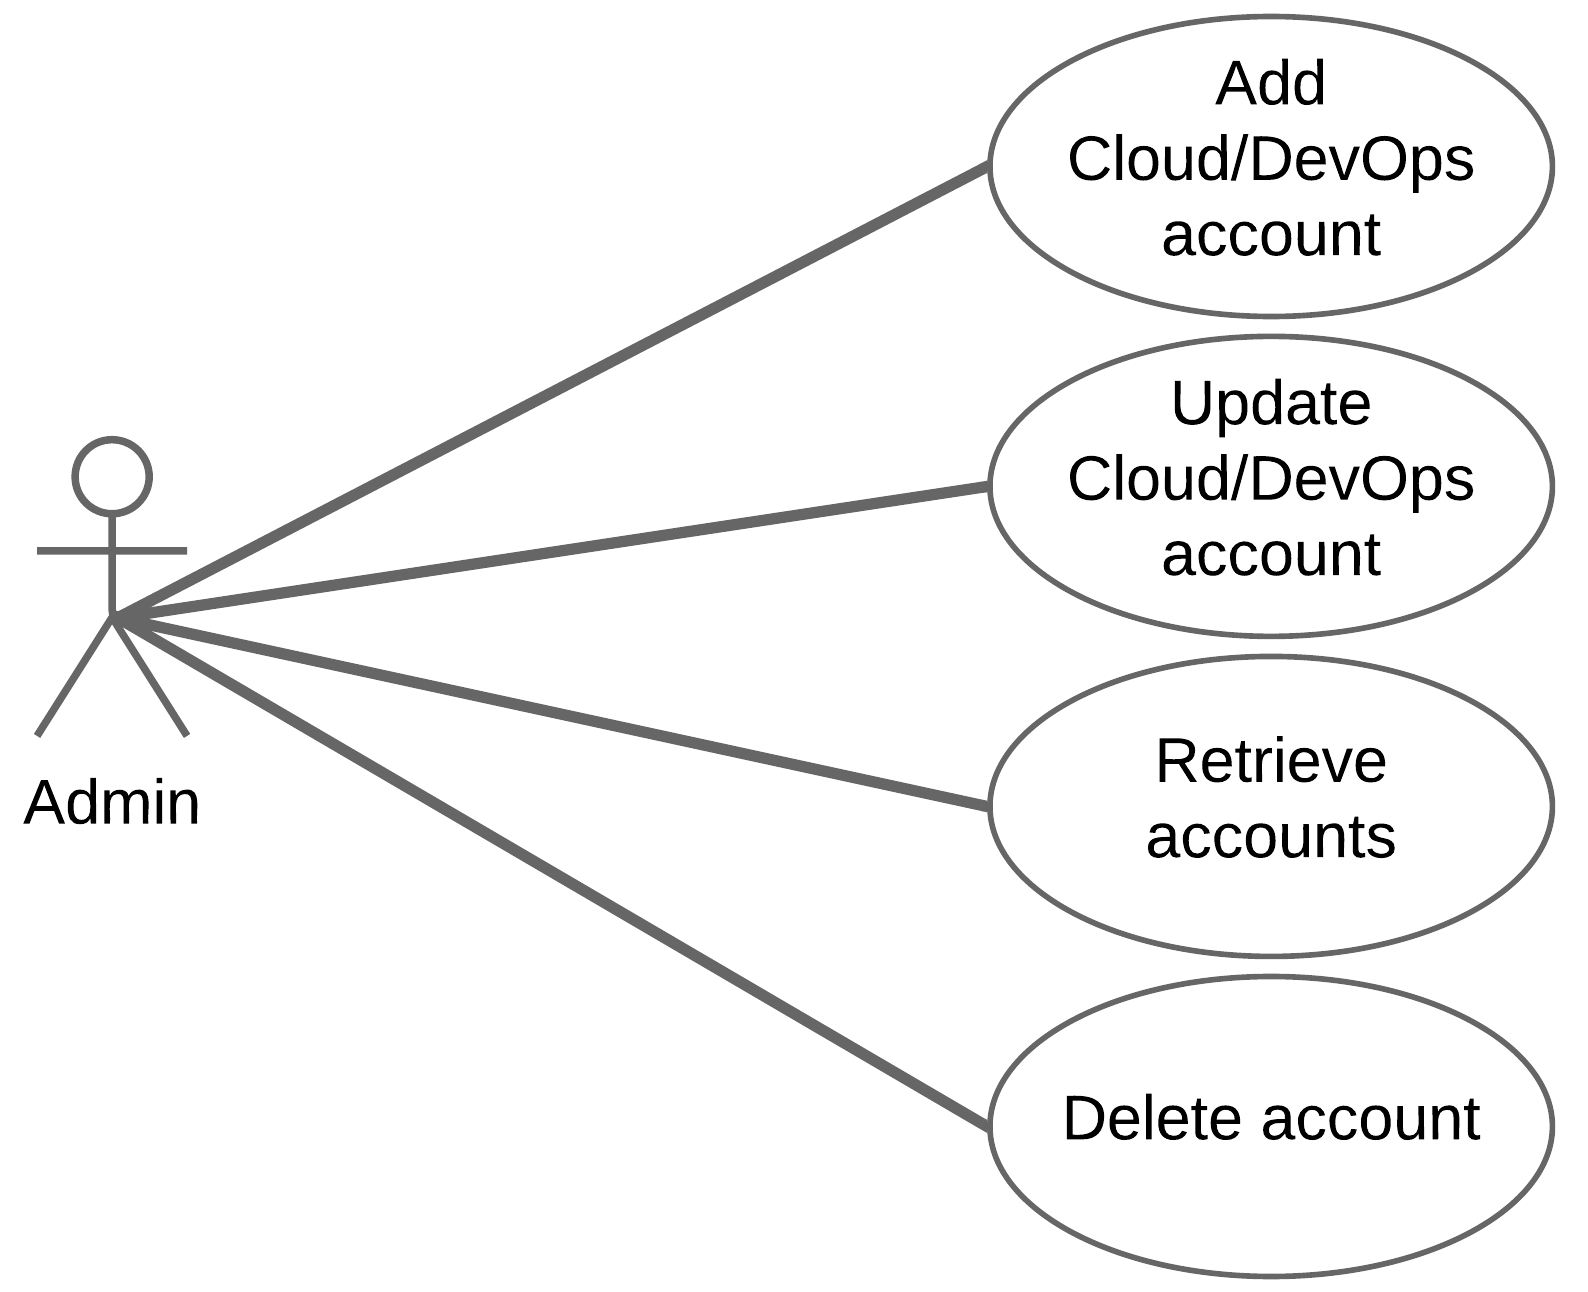
\includegraphics[width=10cm]{use_case-manage_users2}
  \caption{Manage users detailed use case diagram}
  \label{fig:use_case-manage_users2}
\end{figure}

\end{itemize}


\section{Mockups}
In this section, we will outline and confirm the business requirements for the project by presenting UI views 
with the help of mockups. We will begin by introducing the Wireflow tool,
followed by a detailed explanation of the project's mockups.



\subsection{Wireflow}
We suggested using Penpot, an open-source graphical tool for designing user interfaces for websites and
web/desktop/mobile applications. Mockups created with Penpot provide enough interactivity to replace prototypes,
making it easy to collaborate and get feedback on the wireframes. It is defined on their website as \href{https://penpot.app/}{\textit{"Penpot is the web-based open-source design tool that bridges the gap between designers and developers."}}


\subsection{Project mockups}
In this section, we will describe the mockups for our project’s components.

UI General Description:
The dashboard consists of six main screens: main dashboard statistics, instances, storages, vault secrets, clusters, and Docker screens. Below, we will describe the mockups and the requirements for each view.

\subsubsection{Dashboard statistics page}

The figure \hyperref[fig:mockup-dashboard]{\ref{fig:mockup-dashboard}} represents the landing page of our application.
% This page should contain mainly three parts :

% \begin{itemize}
%     \item A chart that represent the changes of counts of negative reviews whether of his topic (shipment, product, website),
%         we termed it as ``store-strength''
%     \item A chart will contain the top used words in positive reviews
%     \item A chart will contain the top used words in negative reviews
% \end{itemize}
All charts should have the export button to different type (PNG, JPEG, PDF,..)
\begin{figure}[h]
  \center
  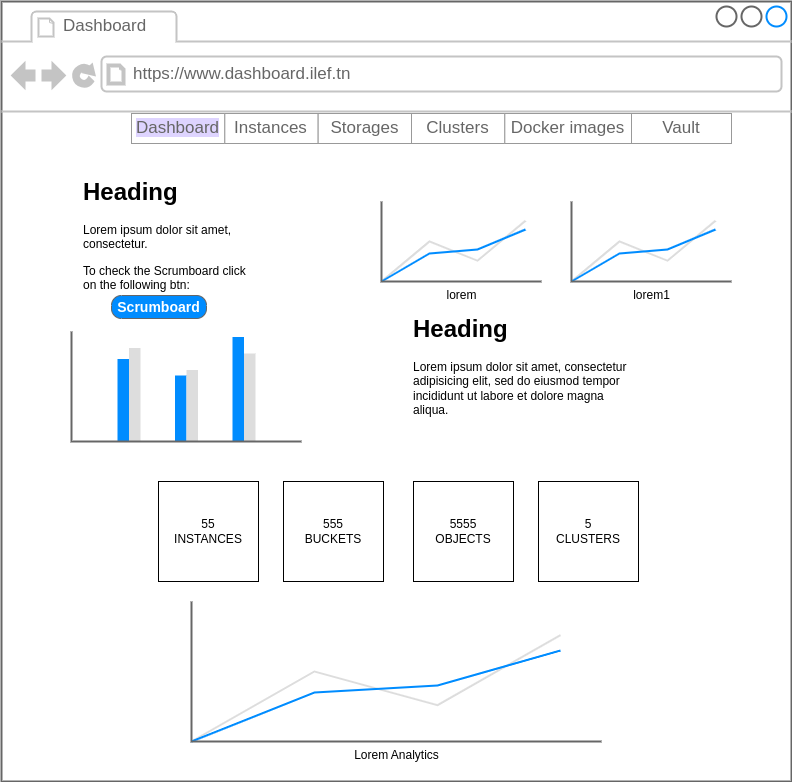
\includegraphics[width=10cm]{mockup-dashboard.png}
  \caption{Main dashboard page mockup}
  \label{fig:mockup-dashboard}
\end{figure}
\vspace{50mm}

\subsubsection{Instances page}

The mockup \hyperref[fig:mockup-instances]{\ref{fig:mockup-instances}} represents the page of instances of our application.

\begin{figure}[h]
  \center
  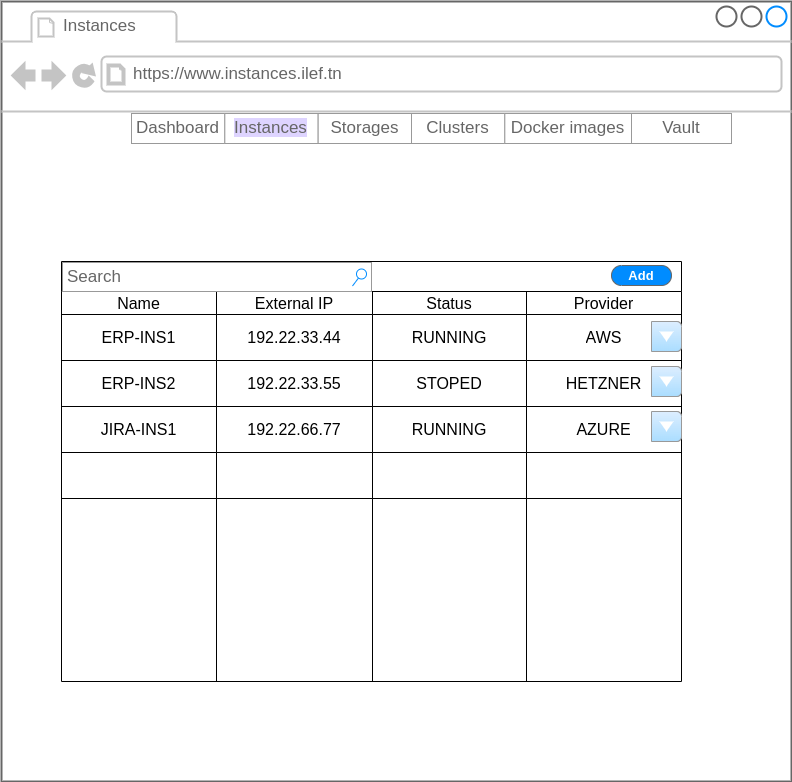
\includegraphics[width=13cm]{mockup-instances.png}
  \caption{Instance page mockup}
  \label{fig:mockup-instances}
\end{figure}
% \vspace{50mm}

\subsubsection{Storages page}

The mockup \hyperref[fig:mockup-storages]{\ref{fig:mockup-storages}} represents the page of storages of our application.
% This screen will present the most important part of Pulpetech-Insights, it should contain mainly two sections.
% The first section include some statistics about reviews and the button of upload new data.
% The second section present the classification table of reviews and the exportation part whether to CSV, XLS or JSON

\begin{figure}[h]
  \center
  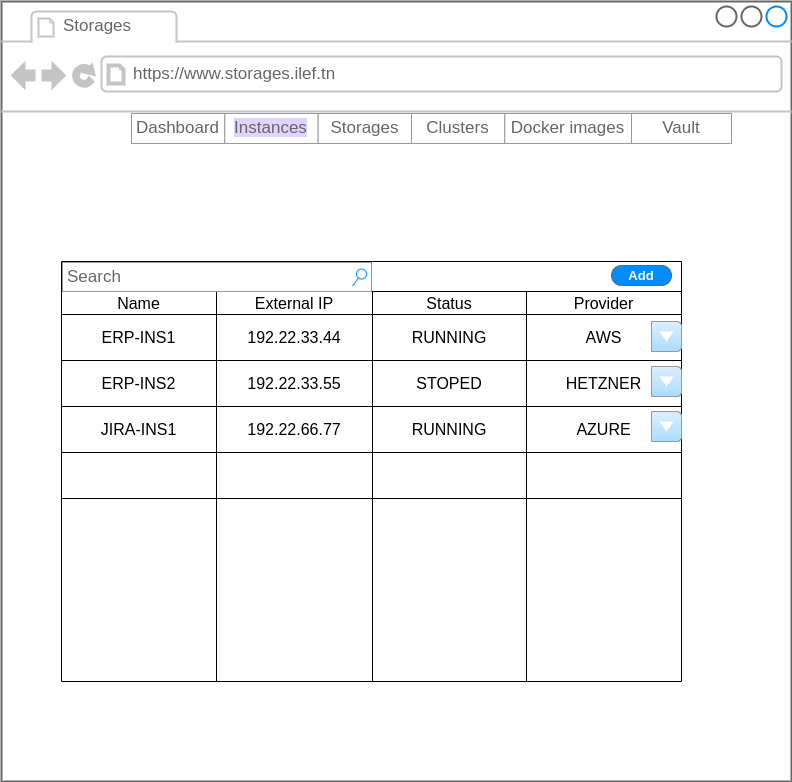
\includegraphics[width=13cm]{mockup-storages.png}
  \caption{Storages page mockup}
  \label{fig:mockup-storages}
\end{figure}

\subsubsection{Docker images page}

% The mockup \hyperref[fig:table]{\ref{fig:table}} represents the page of table of our application.
% This screen will present the most important part of Pulpetech-Insights, it should contain mainly two sections.
% The first section include some statistics about reviews and the button of upload new data.
% The second section present the classification table of reviews and the exportation part whether to CSV, XLS or JSON

% \begin{figure}[h]
%   \center
%   \includegraphics[width=16cm]{table.png}
%   \caption{Table page mockup}
%   \label{fig:table}
% \end{figure}

\subsubsection{Vault secrets page}

% The mockup \hyperref[fig:table]{\ref{fig:table}} represents the page of table of our application.
% This screen will present the most important part of Pulpetech-Insights, it should contain mainly two sections.
% The first section include some statistics about reviews and the button of upload new data.
% The second section present the classification table of reviews and the exportation part whether to CSV, XLS or JSON

% \begin{figure}[h]
%   \center
%   \includegraphics[width=16cm]{table.png}
%   \caption{Table page mockup}
%   \label{fig:table}
% \end{figure}

\subsubsection{Cluster page}

% The mockup \hyperref[fig:table]{\ref{fig:table}} represents the page of table of our application.
% This screen will present the most important part of Pulpetech-Insights, it should contain mainly two sections.
% The first section include some statistics about reviews and the button of upload new data.
% The second section present the classification table of reviews and the exportation part whether to CSV, XLS or JSON

% \begin{figure}[h]
%   \center
%   \includegraphics[width=16cm]{table.png}
%   \caption{Table page mockup}
%   \label{fig:table}
% \end{figure}

% \vspace{20mm}

\section{Product Backlog}

Based on the previous requirements, we derived the product backlog described in Table \ref{tab:product_backlog}.

After the product backlog was established and validated by the Product Owner, the scrum team divided it into four sprints. The sprint durations were suggested by the Scrum Master, with each sprint planned to last one month as shown in Table \ref{tab:sprints_backlog}.

\begin{longtable}{|p{1cm}|p{8cm}|p{2cm}|p{2cm}|}
  \caption{Product Backlogs of Ilef Project} \label{tab:product_backlog} \\
  \hline
  \textbf{ID} & \textbf{User Story} & \textbf{Priority} & \textbf{Estimation (days)} \\
  \hline
  \endfirsthead
  \multicolumn{4}{c}%
  {\tablename\ \thetable\ -- \textit{Continued from previous page}} \\
  \hline
  \textbf{ID} & \textbf{User Story} & \textbf{Priority} & \textbf{Estimation (days)} \\
  \hline
  \endhead
  \hline \multicolumn{4}{r}{\textit{Continued on next page}} \\
  \endfoot
  \hline
  \endlastfoot
  
  1 & As a user, I can log in to the platform securely to access my dashboard and functionalities. & High & 6 \\
  \hline
  2 & As a user, I can view various charts and bar graphs that display statistics and metrics relevant to my cloud resources. & Medium & 9 \\
  \hline
  3 & As a user, I can easily manage instances (create, start, stop, restart, and delete) across different cloud providers (AWS, Azure, GCP, Hetzner). & High & 10 \\
  \hline
  4 & As a user, I can manage storage solutions, including uploading, fetching, and deleting objects, across different cloud providers (AWS, Azure, GCP). & High & 10 \\
  \hline
  5 & As a user, I can quickly deploy a Docker image to a virtual machine instance. & Medium & 6 \\
  \hline
  6 & As a user, I can create a Kubernetes cluster from a Docker image for container orchestration. & Medium & 15 \\
  \hline
  7 & As a user, I can manage and retrieve secrets from the vault server securely. & High & 12 \\
  \hline
  8 & As a user, I can fetch Docker images stored in the Nexus repository for deployment. & Medium & 6 \\
  \hline
  9 & As a user, I can use the integrated Scrumboard to manage and track project tasks and progress. & Medium & 5 \\
  \hline
  10 & As an admin, I can manage user accounts, including creating, modifying, and deleting accounts, and assigning roles and permissions. & High & 8 \\
  \hline
  
  \end{longtable}

\begin{table}[h!]
\centering
\caption{User Stories through each sprint}
\label{tab:sprints_backlog}
\begin{tabular}{|p{2cm}|p{10cm}|p{2cm}|}
\hline
\textbf{Sprint} & \textbf{User Stories} & \textbf{Estimation (days)} \\ \hline
Sprint 1 & As a user, I can log in to the platform securely to access my dashboard and functionalities. & 6 \\ \cline{2-3}
 & As a user, I can view various charts and bar graphs that display statistics and metrics relevant to my cloud resources. & 9 \\ \cline{2-3}
 & As a user, I can use the integrated Scrumboard to manage and track project tasks and progress. & 5 \\ \hline

\multirow{2}{*}{Sprint 2} & As a user, I can easily manage instances (create, start, stop, restart, and delete) across different cloud providers (AWS, Azure, GCP, Hetzner). & 10 \\ \cline{2-3}
 & As a user, I can manage storage solutions, including uploading, fetching, and deleting objects, across different cloud providers (AWS, Azure, GCP). & 10 \\ \hline

\multirow{3}{*}{Sprint 3} & As a user, I can quickly deploy a Docker image to a virtual machine instance. & 6 \\ \cline{2-3}
 & As a user, I can create a Kubernetes cluster from a Docker image for container orchestration. & 8 \\ \cline{2-3}
 & As a user, I can fetch Docker images stored in the Nexus repository for deployment. & 6 \\ \hline

\multirow{2}{*}{Sprint 4} & As a user, I can manage and retrieve secrets from the vault server securely. & 12 \\ \cline{2-3}
 & As an admin, I can manage user accounts, including creating, modifying, and deleting accounts, and assigning roles and permissions. & 8 \\ \hline
\end{tabular}
\end{table}
% \begin{table}[!htbp]
% \centering
% \label{sprints}
% \begin{tabular}{|p{3cm}|p{8cm}|p{2cm}|p{2cm}|}
%                            \hline
%                               &  User stories & Estimation & Priority \\ \hline
%     Sprint 1                     & As a user, I want to be able to predict the review polarity  & 15 & 1 \\
%     \cline{2-4}
%     {} &  As a user, I want to be able to predict the review polarity  & 15 & 2

%     \\ \hline
%                          &  As a user, I want to login using my username and password and start using the application right away. &  15 & 3
%     \\ \cline{2-4} 
%     {\multirow{2}{*}{}} {} &  As a user, I want to see the result of classification table of reviews.  &  7 & 4
%     \\ \cline{2-4}
%     {}                            &  As an administrator, I want to be able to manage all reviews and users accounts. &  10 & 5
%     \\ \cline{2-4} 


%     {\multirow{3}{*}{}} Sprint 2  & As a user, I want to visualize the charts describe the reviews & 9 & 6
%     \\ \cline{2-4}
%     {}                            & As a user, I want to be able to filter data from a data table based on multiple conditions.&  4 & 7
%     \\ \cline{2-4}
%     {\multirow{3}{*}{}}{}  & As a user, I want to be able to upload reviews to be part of database. & 7 & 8
%     \\ \cline{2-4}
%     {}                            & As a user, I want to read a summary of the sentiment analysis of reviews. & 4 & 9    \\
%     \cline{2-4}
%     {}                            &  As a user, I want to export the charts and the table content to different types. &  4 & 10\\ \hline

% \end{tabular}
% \caption{Product Backlog and User Stories through each sprint}
% \end{table}

% The table \hyperref[sprints]{3.2}  defines the Product Backlog and the user stories that will be achieved during each sprint




\section*{Conclusion}
In this chapter, we have conducted a thorough requirements analysis and defined the specifications needed.
This process allowed us to clearly identify the system's actors and the features it must implement. Additionally,
we have created mockups of the current system and described the functionalities required by the user.